%%%%%%%%%%%%%%%%%%%%%%%%%%%%%%%%%%%%%%%%%%%%%%%%%%%%%%%%%%%%%%%%%%%%%%%%%%%%%%%%
%
% Template license:
% CC BY-NC-SA 3.0 (http://creativecommons.org/licenses/by-nc-sa/3.0/)
%
%%%%%%%%%%%%%%%%%%%%%%%%%%%%%%%%%%%%%%%%%%%%%%%%%%%%%%%%%%%%%%%%%%%%%%%%%%%%%%%%

%----------------------------------------------------------------------------------------
%	PACKAGES AND OTHER DOCUMENT CONFIGURATIONS
%----------------------------------------------------------------------------------------

\documentclass[
11pt, % The default document font size, options: 10pt, 11pt, 12pt
%oneside, % Two side (alternating margins) for binding by default, uncomment to switch to one side
%chapterinoneline,% Have the chapter title next to the number in one single line
spanish,
singlespacing, % Single line spacing, alternatives: onehalfspacing or doublespacing
%draft, % Uncomment to enable draft mode (no pictures, no links, overfull hboxes indicated)
%nolistspacing, % If the document is onehalfspacing or doublespacing, uncomment this to set spacing in lists to single
%liststotoc, % Uncomment to add the list of figures/tables/etc to the table of contents
%toctotoc, % Uncomment to add the main table of contents to the table of contents
parskip, % Uncomment to add space between paragraphs
%codirector, % Uncomment to add a codirector to the title page
headsepline, % Uncomment to get a line under the header
]{MastersDoctoralThesis} % The class file specifying the document structure



%----------------------------------------------------------------------------------------
%	INFORMACIÓN DE LA MEMORIA
%----------------------------------------------------------------------------------------

\thesistitle{Sistema de riego autónomo aplicado a la agricultura} % El títulos de la memoria, se usa en la carátula y se puede usar el cualquier lugar del documento con el comando \ttitle

% Nombre del posgrado, se usa en la carátula y se puede usar el cualquier lugar del documento con el comando \degreename
\posgrado{Carrera de Especialización en Sistemas Embebidos} 
%\posgrado{Carrera de Especialización en Internet de las Cosas} 
%\posgrado{Carrera de Especialización en Intelegencia Artificial}
%\posgrado{Maestría en Sistemas Embebidos} 
%\posgrado{Maestría en Internet de las cosas}

\author{Ing. Jhonny Velasco Collazos} % Tu nombre, se usa en la carátula y se puede usar el cualquier lugar del documento con el comando \authorname

\director{Ing. Luis Mariano Campos (FIUBA)} % El nombre del director, se usa en la carátula y se puede usar el cualquier lugar del documento con el comando \dirname
%\codirector{Nombre del codirector (pertenencia)} % El nombre del codirector si lo hubiera, se usa en la carátula y se puede usar el cualquier lugar del documento con el comando \codirname.  Para activar este campo se debe descomentar la opción "codirector" en el comando \documentclass, línea 23.

\juradoUNO{Nombre del jurado 1 (pertenencia)} % Nombre y pertenencia del un jurado se usa en la carátula y se puede usar el cualquier lugar del documento con el comando \jur1name
\juradoDOS{Nombre del jurado 2 (pertenencia)} % Nombre y pertenencia del un jurado se usa en la carátula y se puede usar el cualquier lugar del documento con el comando \jur2name
\juradoTRES{Nombre del jurado 3 (pertenencia)} % Nombre y pertenencia del un jurado se usa en la carátula y se puede usar el cualquier lugar del documento con el comando \jur3name

%\ciudad{Ciudad Autónoma de Buenos Aires}
\ciudad{ciudad de Lima}

\fechaINICIO{marzo de 2023}
\fechaFINAL{Mayo de 2023}


\keywords{Sistemas embebidos, FIUBA} % Keywords for your thesis, print it elsewhere with \keywordnames


\begin{document}


\frontmatter % Use roman page numbering style (i, ii, iii, iv...) for the pre-content pages

\pagestyle{plain} % Default to the plain heading style until the thesis style is called for the body content


%----------------------------------------------------------------------------------------
%	RESUMEN - ABSTRACT 
%----------------------------------------------------------------------------------------

\begin{abstract}
\addchaptertocentry{\abstractname} % Add the abstract to the table of contents
%
%The Thesis Abstract is written here (and usually kept to just this page). The page is kept centered vertically so can expand into the blank space above the title too\ldots
\centering

Esta memoria describe el proceso de diseño y fabricación de un prototipo de un sistema de riego autónomo con conectividad inalámbrica. Este prototipo pretende ayudar a los agricultores o personas amantes de las plantas, a monitorear y automatizar el proceso de riego y a su vez mejorar eficiencias y reducción de costos en los procesos operativos.

Para poder llevar adelante este trabajo, fue indispensable la aplicación de conocimientos técnicos que se desarrollaron durante la carrera como los protocolos de comunicación en sistemas embebidos, diseño de circuitos impresos, desarrollo de aplicaciones de tiempo real, entre otros.

\end{abstract}

%----------------------------------------------------------------------------------------
%	CONTENIDO DE LA MEMORIA  - AGRADECIMIENTOS
%----------------------------------------------------------------------------------------

\begin{acknowledgements}
%\addchaptertocentry{\acknowledgementname} % Descomentando esta línea se puede agregar los agradecimientos al índice
\vspace{1.5cm}

A mi familia, por creer en mí.

A Yessica, por su apoyo incondicional.

A mi director, Ing. Luis Mariano Campos, por su buena predisposición y calidad profesional.

A todos ellos, muchas gracias.

\end{acknowledgements}

%----------------------------------------------------------------------------------------
%	LISTA DE CONTENIDOS/FIGURAS/TABLAS
%----------------------------------------------------------------------------------------

\tableofcontents % Prints the main table of contents

\listoffigures % Prints the list of figures

\listoftables % Prints the list of tables


%----------------------------------------------------------------------------------------
%	CONTENIDO DE LA MEMORIA  - DEDICATORIA
%----------------------------------------------------------------------------------------

\dedicatory{\textbf{Dedicado a mi familia.}}  % escribir acá si se desea una dedicatoria

%----------------------------------------------------------------------------------------
%	CONTENIDO DE LA MEMORIA  - CAPÍTULOS
%----------------------------------------------------------------------------------------

\mainmatter % Begin numeric (1,2,3...) page numbering

\pagestyle{thesis} % Return the page headers back to the "thesis" style

% Incluir los capítulos como archivos separados desde la carpeta Chapters

% Chapter 1

\chapter{Introducción general} % Main chapter title

\label{Chapter1} % For referencing the chapter elsewhere, use \ref{Chapter1} 
\label{IntroGeneral}

%----------------------------------------------------------------------------------------

% Define some commands to keep the formatting separated from the content 
\newcommand{\keyword}[1]{\textbf{#1}}
\newcommand{\tabhead}[1]{\textbf{#1}}
\newcommand{\code}[1]{\texttt{#1}}
\newcommand{\file}[1]{\texttt{\bfseries#1}}
\newcommand{\option}[1]{\texttt{\itshape#1}}
\newcommand{\grados}{$^{\circ}$}

%----------------------------------------------------------------------------------------

Esta sección presenta las motivaciones, alcance y objetivos así como la comparativa de productos similares en el mercado.

%----------------------------------------------------------------------------------------
\section{Motivación}

En muchas zonas del Perú, los pequeños agricultores se ven afectados por los fenómenos ambientales como las sequías y heladas que repercuten directamente en sus cosechas. Por otro lado, constantemente realizan muchas operaciones manuales que podrían automatizarse para generar eficiencias en el uso de los recursos.

Uno de los principales fenómenos que afecta mucho a la producción agrícola son las heladas, normalmente este fenómeno se produce durante las madrugadas dañando toda la cosecha. Una forma eficaz de proteger los sembríos de las heladas es detectar a tiempo el fenómeno y luego rociar abundante agua en la zona.

Es por esa razón que el espíritu de este prototipo es poner al alcance de los pequeños agricultores un sistema de riesgo autónomo que permita automatizar los procesos de riego y tener la capacidad de monitorear las diferentes variables ambientales para tomar una acción correctiva.

%----------------------------------------------------------------------------------------

\section{Alcance y objetivos}

Esta memoria describe el proceso de diseño y fabricación de un prototipo de un sistema de riego autónomo con conectividad inalámbrica que permita controlar dos (4) electroválvulas independientes y una (1) motobomba para mayor presión en el flujo de agua. Asimismo, el sistema estará equipado por sensores de presión atmosférica, temperatura y humedad ambiental.

La información será visible a través de una pantalla LCD y tendrá un joystick de dos ejes para su control. También dispondrá de un \textit{Real Time Clock} (RTC) para contabilizar el tiempo.

Como parte del alcance se ha contemplado lo siguiente:

\begin{enumerate}
	\item Diseño del \textit{hardware} del sistema de riego autónomo.
	\item Diseño de la \textit{PCB}.
	\item Ensamblaje.
	\item Diseño del \textit{firmware} del sistema de riego autónomo basado en el microcontrolador ESP32 o similar.
	\item Diseño de la caja 3D.
	\item Pruebas.
\end{enumerate}

El presente prototipo en esta primera etapa no incluye:
\begin{enumerate}
	\item Diseño e implementación de la arquitectura nube donde estarán alojados la API, aplicación web y servidor MQTT.
	\item Diseño e implementación de la API que se comunicará con la aplicación web o móvil.
	\item Diseño e implementación de la aplicación web o móvil para control remoto de los parámetros.
	\item Actualización del \textit{firmware} del microcontrolador para que soporte la comunicación MQTT con el \textit{broker}.
	\item Diseño e implementación de sensores externos e inalámbricos para monitorear la temperatura y humedad de la tierra.
\end{enumerate}

Para el desarrollo del presente proyecto se supone que:
\begin{enumerate}
\item Se importará de China los siguientes componentes electrónicos:
	\begin{itemize}
	\item Un microcontrolador ESP32 o similar.
	\item Un convertidor USB a TTL UART.
	\item Un chip DS3231 ''\textit{Real Time Clock}'' o similar.
	\item Una pantalla LCD de 2.4'' o 3.5''.
	\item Un sensor de temperatura, humedad y presión atmosférica (BME280) o similar.
	\item Un \textit{joystick} de 2 ejes (x-y).
	\item Otros componentes: resistencias, capacitores, diodos, etc.
	\end{itemize}	
\item Se dispondrá de un mínimo de 704 horas requeridas para realizar el prototipo.
\item Se dispondrá del presupuesto económico para realizar las compras requeridas.
\item Se dispondrá del \textit{software} requerido para el prototipo: IDE del microcontrolador, KiCad 6 y Autodesk Fusion360.
\item Se dispondrá de un proveedor para la elaboración de la PCB.
\item Se dispondrá de un proveedor local para las impresiones 3D de la carcasa.
\end{enumerate}

%----------------------------------------------------------------------------------------
\newpage
\section{Estado del arte}

En la actualidad podemos encontrar diferentes empresas que comercializan programadores de riego o \textit{timers} que cumplen dicha función. Sin embargo en muchos de los casos son dispositivos muy generales y con poca flexibilidad.
\newline
\begin{table}[h]
	\begin{center}
		\begin{tabular}{ p{1cm} p{2cm} p{3cm} p{2cm} p{2cm} }

			\hline 
	 		\textbf{Item} & \textbf{Marca}  & \textbf{Modelo} & \textbf{Precio} & \textbf{Salidas}	\\
			\hline 
			1 & Rain Bird & 1ZEHTMR & S/ 295.00 & 1 salida	\\
			2 & Rain Bird & ESP-RZXe & S/ 480.00  & 8 salidas	\\
			3 & Rain Bird & TM2-6-230 & S/ 658.00  & 6 salidas	\\
			4 & Rain Bird & TM2-12-230 & S/ 1561.00  & 12 salidas	\\
			5 & HUNTER & BTT101 & S/ 300.00  & 1 salida	\\
			6 & GALCON & 80024/8 & S/ 765.00  & 8 salidas	\\
			\hline 
		\end{tabular}
		\caption{Tabla comparativa de fabricantes de programadores de riego o similares}
	\end{center}
\end{table}

\begin{figure}[h]
	\centering
	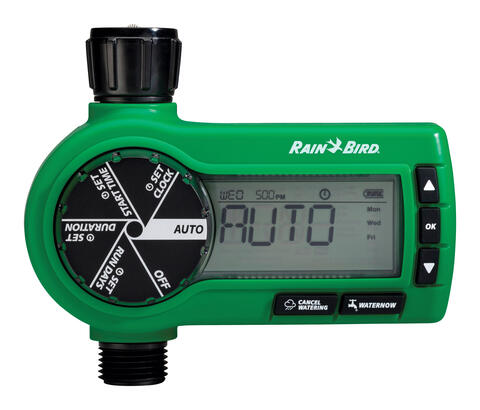
\includegraphics[width=0.4\textwidth]{1ZEHTMR}
	\caption{Rain Bird 1ZEHTMR.}
\end{figure}

\begin{figure}[h]
	\centering
	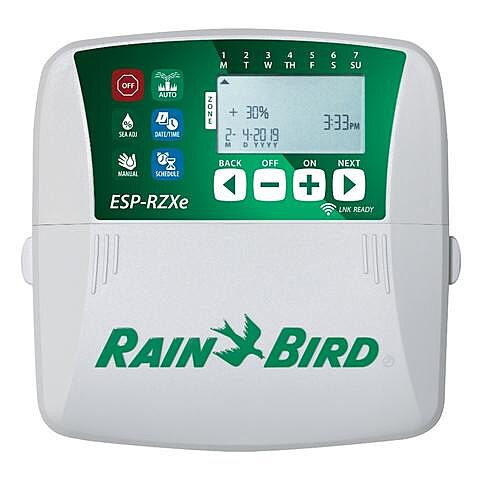
\includegraphics[width=0.4\textwidth]{ESP-RZXe}
	\caption{Rain Bird ESP-RZXe.}
\end{figure}

\begin{figure}[h]
	\centering
	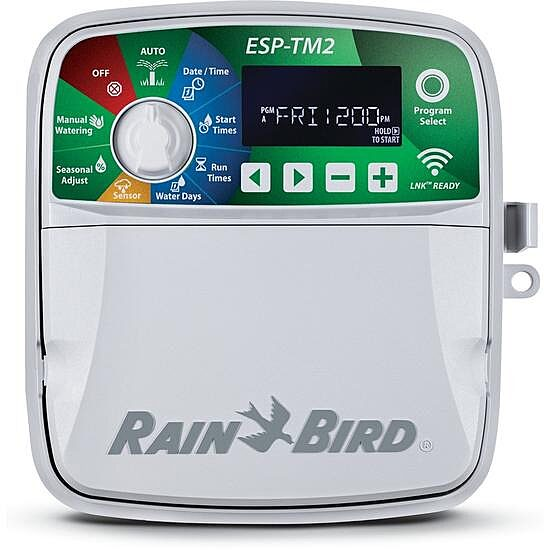
\includegraphics[width=0.4\textwidth]{ESP TM2-X-230}
	\caption{Rain Bird ESP TM2-X-230.}
\end{figure}

\begin{figure}[h]
	\centering
	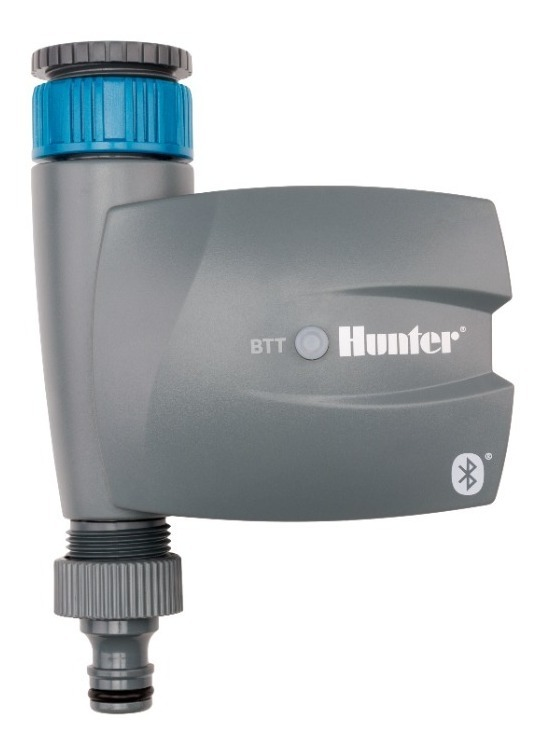
\includegraphics[width=0.4\textwidth]{BTT101}
	\caption{Hunter BTT101.}
\end{figure}

\begin{figure}[h]
	\centering
	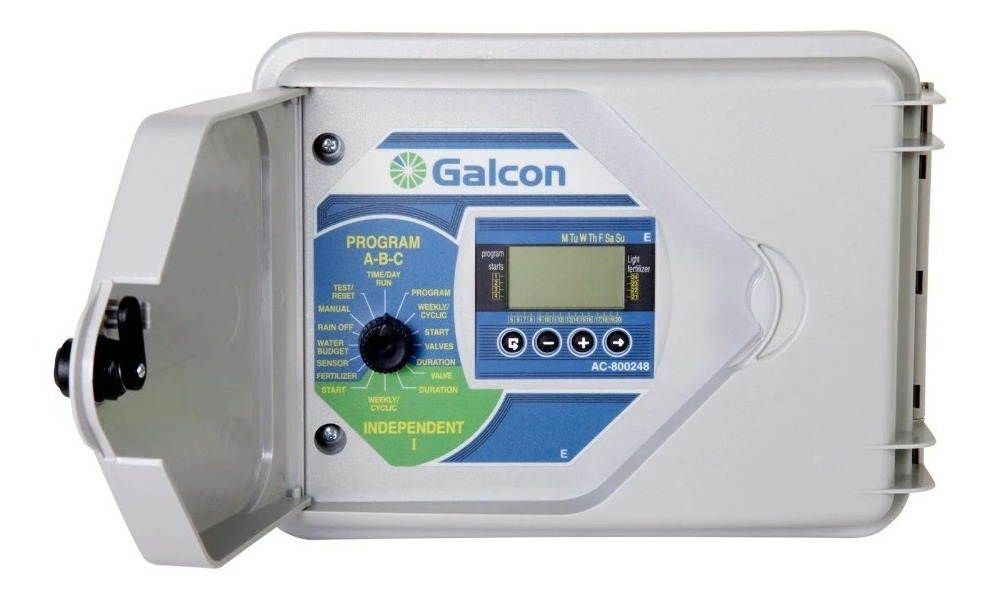
\includegraphics[width=0.4\textwidth]{80024-8}
	\caption{Galcon 80024-8.}
\end{figure}
%----------------------------------------------------------------------------------------

\chapter{Introducción específica} % Main chapter title

\label{Chapter2}

%----------------------------------------------------------------------------------------
%	SECTION 1
%----------------------------------------------------------------------------------------
Esta sección presenta los requerimientos acordados con el cliente, las diferentes tecnologías a utilizar y las herramientas y recursos utilizados para realizar el trabajo.

\section{Requerimientos acordados con el cliente}
\subsection{Requerimientos funcionales:}
	\begin{itemize}
		\item \textbf{Requerimientos de \textit{hardware}:}
			\begin{enumerate}
				\item El dispositivo deberá contar con un transformador de 110 / 220 VAC a 24 VAC a 2 A que será utilizado para alimentar el microcontrolador, sensores y periféricos de entrada y salida.
				\item El dispositivo deberá contar con un rectificador y regulador de tensión a 5 VDC y 3.3 VDC.
				\item El dispositivo deberá contar con una interface USB para su programación, actualización de código y depuración.
				\item El dispositivo deberá contar con una pantalla LCD o similar de mínimo 2.4'' hasta 3.5''.
				\item El dispositivo deberá contar con un \textit{joystick} o botoneras para su manipulación y configuración.
				\item El dispositivo deberá contar con un \textit{Real Time Clock} (RTC), el mismo que deberá mantener la fecha y hora actual ante un corte de energía.
				\item El dispositivo deberá contar con un sensor de temperatura que mida mínimo en el rango de -20 °C a 60 °C con una precisión de +/- 1 °C o inferior.
				\item El dispositivo deberá contar con un sensor de humedad relativa de 0-100 \% con una precisión de +/- 3 \% o inferior.
				\item El dispositivo deberá contar con un sensor de presión atmosférica que mida en el rango de 300 a 1100 hPa (0.3 - 1.1 bar) con una precisión absoluta de +/- 1 hPa o inferior.
				\item El dispositivo deberá contar con cuatro (4) salidas independientes para las electroválvulas de 24 VAC y las mismas que deberán ser energizadas por el propio transformador del dispositivo.
				\item El dispositivo deberá contar con una (1) salida independiente para la motobomba.
				\item El dispositivo deberá soportar la tecnología Wi-Fi para envío y recepción de datos.	
			\end{enumerate}
			
		\item \textbf{Requerimientos de \textit{firmware}:}
			\begin{enumerate}	
				\item Se deberá usar el idioma español o ingles.
				\item La pantalla LCD debe mostrar el menú de opciones de configuración:
					\begin{itemize}
						\item Establecer fecha y hora
						\item Programar secuencias de riego
						\item Riego manual
						\item Activar/Desactivar válvulas
					\end{itemize}
				\item Se debe permitir establecer la fecha y hora a través del \textit{joystick} o botoneras, el formato a utilizar será de 24 hrs.
				\item Se debe permitir programar las secuencias de riego de cada electroválvula de manera independiente siguiendo las siguientes consideraciones:
					\begin{itemize}
						\item Configurar la hora de ejecución de riego en horas, minutos y segundos.
						\item Configurar la duración de riego en horas, minutos y segundos.
						\item Configurar la frecuencia expresado en horas y minutos. Por ejemplo, ejecutar el riego cada 2 horas.
						\item Seleccionar los días de riego.
						\item Poder borrar la configuración actual de la secuencia de riego.
					\end{itemize}		
				\item Se debe permitir encender cada electroválvula de manera manual independientemente de la programación que tenga configurada.
				\item Se debe permitir activar y desactivar cada secuencia de riego de manera independiente.
				\item La pantalla LCD debe mostrar un \textit{dashboard} con la siguiente información:
					\begin{itemize}
						\item La fecha y hora actual.
						\item La programación actual de las secuencias de riego.
						\item La presión atmosférica (altitud).
						\item La temperatura y humedad ambiental.
						\item El estado de los sensores de nivel de agua de los tanques.
						\item El estado de las electroválvulas (encendidas/apagadas).
					\end{itemize}
			\end{enumerate}
	\end{itemize}

\subsection{Requerimientos no funcionales:}
	\begin{enumerate}
		\item El tiempo de muestreo de los sensores de temperatura, humedad y presión atmosférica será de 5 segundos como máximo.
		\item Se debe garantizar un soporte post venta de 5 años.
	\end{enumerate}

\subsection{Historias de usuario}
\label{sec:backlog}
Para la ponderación de la dificultad, complejidad e incertidumbre de las historias de usuarios se usará la serie de Fibonacci y se clasificará en tres niveles: 
\begin{itemize}
\item Baja (1)
\item Media (3)
\item Alta (5).
\end{itemize}

El puntaje total será redondeado hacia arriba al valor mas cercano de la serie de Fibonacci. Por ejemplo, si la sumatoria da como resultado 11, el Story Point a considerar será 13.

\textbf{Historia 1:}
''Como operario, quiero que el idioma del dispositivo sea español por un tema de facilidad de uso''.
\begin{itemize}
\item \textbf{Dificultad:} baja (1)
\item \textbf{Complejidad:} baja (1)
\item \textbf{Incertidunbre:} baja (1)
\newline
\newline
\textbf{\textit{Story Point}: 3}
\end{itemize}

\textbf{Historia 2:}
''Como agricultor, quiero poder visualizar el día, mes, año, hora, minuto, temperatura, humedad y presión atmosférica (altitud) en tamaño visible''.
\begin{itemize}
\item \textbf{Dificultad:} alta (5)
\item \textbf{Complejidad:} media (3)
\item \textbf{Incertidunbre:} media (3)
\newline
\newline
\textbf{\textit{Story Point:} 13}
\end{itemize}

\textbf{Historia 3:}
''Como agricultor, quiero tener la posibilidad de programar los riegos una vez al día o varias veces al día, un vez a la semana o varios días a la semana''.
\begin{itemize}
\item \textbf{Dificultad:} alta (5)
\item \textbf{Complejidad:} alta (5)
\item \textbf{Incertidunbre:} media (3)
\newline
\newline
\textbf{\textit{Story Point:} 13}
\end{itemize}

\textbf{Historia 4:}
''Como operario, quiero que en caso sea necesario usar una motobomba, esta última se active después de haberse iniciado la secuencia de riego''.
\begin{itemize}
\item \textbf{Dificultad:} media (3)
\item \textbf{Complejidad:} baja (1)
\item \textbf{Incertidunbre:} baja (1)
\newline
\newline
\textbf{\textit{Story Point:} 5}
\end{itemize}

\textbf{Historia 5:}
''Como operario, quiero que cuando haya transcurrido el tiempo de riego, primero se apague la motobomba y después se cierren las electroválvulas para evitar daños en la motobomba''.
\begin{itemize}
\item \textbf{Dificultad:} media (3)
\item \textbf{Complejidad:} baja (1)
\item \textbf{Incertidunbre:} baja (1)
\newline
\newline
\textbf{\textit{Story Point:} 5}
\end{itemize}

\textbf{Historia 6:}
''Como agricultor, quiero que el dispositivo tenga la capacidad de controlar una motobomba para darle mayor presión al agua en caso sea necesario.
\begin{itemize}
\item \textbf{Dificultad:} baja (1)
\item \textbf{Complejidad:} baja (1) 
\item \textbf{Incertidunbre:} baja (1) 
\newline
\newline
\textbf{\textit{Story Point:} 3}
\end{itemize}

\textbf{Historia 7:}
''Como agricultor, quisiera que el dispositivo incluya sus propias electroválvulas para evitarme el trabajo de buscar esas partes fuera y/o tener problemas de incompatibilidad.
\begin{itemize}
\item \textbf{Dificultad:} baja (1)
\item \textbf{Complejidad:} baja (1)
\item \textbf{Incertidunbre:} baja (1)
\newline
\newline
\textbf{\textit{Story Point:} 3}
\end{itemize}

\textbf{Historia 8:}
''Como operario, quisiera poder activar de forma voluntaria las electroválvulas e iniciar una secuencia de riego manual sin depender y desconfigurar la secuencia de riego programada.
\begin{itemize}
\item \textbf{Dificultad:} media (3)
\item \textbf{Complejidad:} media (3)
\item \textbf{Incertidunbre:} baja (1)
\newline
\newline
\textbf{\textit{Story Point:} 8}
\end{itemize}

\textbf{Historia 9:}
''Como agricultor, quisiera poder deshabilitar la secuencia de riego de manera temporal sin borrar la configuración ya establecida. Esto sería útil cuando se tenga que realizar algún mantenimiento en las cañerías o durante las temporadas de cosecha.
\begin{itemize}
\item \textbf{Dificultad:} baja (1) 
\item \textbf{Complejidad:} media (3) 
\item \textbf{Incertidunbre:} baja (1) 
\newline
\newline
\textbf{\textit{Story Point:} 5}
\end{itemize}

\section{Tecnologías utilizadas}
\subsection{ESP32:}
Como cerebro del dispositivo se utilizó el \textit{System on a Chip} ESP32 del fabricante Espressif. El ESP32 emplea un microprocesador Tensilica Xtensa LX6 de doble núcleo.

\begin{figure}[h]
	\centering
	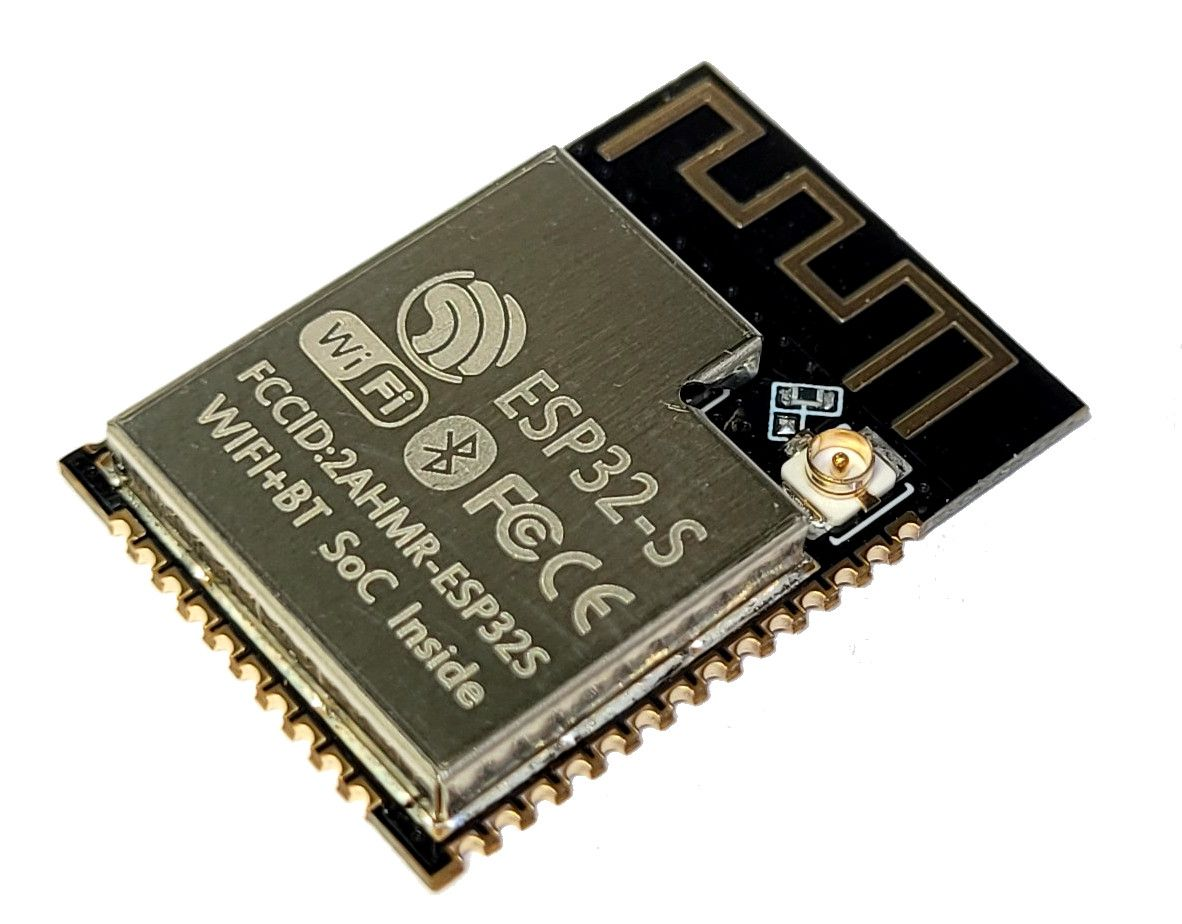
\includegraphics[width=0.4\textwidth]{SoC ESP32}
	\caption{System on a Chip Espressif ESP32}
\end{figure}

Entre las principales características del ESP32 son:
\begin{enumerate}
	\item Procesador:
	\begin{enumerate}
		\item CPU: microprocesador de 32-bit Xtensa LX6 de doble núcleo (o de un solo núcleo), operando a 160 o 240 MHz y rindiendo hasta 600 DMIPS.
		\item Co-procesador de ultra baja energía (ULP).
	\end{enumerate}
	\item Memoria: 520 KiB SRAM.
	\item Conectividad inalámbrica:
	\begin{enumerate}
		\item Wi-Fi: 802.11 b/g/n.
		\item Bluetooth: v4.2 BR/EDR y BLE.
	\end{enumerate}
	\item Periféricos:
	\begin{enumerate}
		\item 12-bit SAR ADC de hasta 18 canales.
		\item 2 × 8-bit DACs.
		\item 10 × sensores de tacto (sensores capacitivos GPIOs).
		\item 4 × SPI.
		\item 2 × interfaces I²S.
		\item 2 × interfaces I²C.
		\item 3 × UART
		\item Controlador host SD/SDIO/CE-ATA/MMC/eMMC
		\item Controlador esclavo SDIO/SPI
		\item Interfaz Ethernet MAC con DMA dedicado y soporte para el protocolo IEEE 1588 Precision Time Protocol.
		\item Bus CAN 2.0.
		\item Controlador remoto infrarrojo (TX/RX, hasta 8 canales).
		\item Motor PWM.
		\item LED PWM (hasta 16 canales).
		\item Sensor de efecto Hall
		\item Pre-amplificador analógico de ultra baja potencia
	\end{enumerate}
	\item Seguridad:
	\begin{enumerate}
		\item Soporta todas las características de seguridad estándar de IEEE 802.11, incluyendo WFA, WPA/WPA2 y WAPI.
		\item Arranque seguro.
		\item Cifrado flash.
		\item 1024-bit OTP, hasta 768-bit para clientes.
		\item Criptografía acelerada por hardware: AES, SHA-2, RSA, criptografía de curva elíptica (ECC), generador de números aleatorios (RNG).
	\end{enumerate}	
\end{enumerate}



\subsection{Pantalla TFT de 3.5 pulgadas:}

\subsection{Joystick:}

\subsection{Sensor BME280:}

\subsection{Chip FT232RL:}

\section{Herramientas y recursos de terceros}

 
\include{Chapters/Chapter3}
\include{Chapters/Chapter4} 
\include{Chapters/Chapter5} 

%----------------------------------------------------------------------------------------
%	CONTENIDO DE LA MEMORIA  - APÉNDICES
%----------------------------------------------------------------------------------------

\appendix % indicativo para indicarle a LaTeX los siguientes "capítulos" son apéndices

% Incluir los apéndices de la memoria como archivos separadas desde la carpeta Appendices
% Descomentar las líneas a medida que se escriben los apéndices

%\include{Appendices/AppendixA}
%\include{Appendices/AppendixB}
%\include{Appendices/AppendixC}

%----------------------------------------------------------------------------------------
%	BIBLIOGRAPHY
%----------------------------------------------------------------------------------------

\Urlmuskip=0mu plus 1mu\relax
\raggedright
\printbibliography[heading=bibintoc]

%----------------------------------------------------------------------------------------

\end{document}  
